\section{Experimental Study}
\label{sec-exp}

We evaluate \sys along four research questions.
\begin{itemize}
\item \textbf{[RQ1] The store}: how does a B+ tree store of three permutations
  compare with an LSM, a Java B+ tree, and a relational store on triple
  patterns, queries, and loading?
\item \textbf{[RQ2] Hierarchies and the plan rewrite}: what do the interval labels
  and the entailment rewrite cost and buy against materializing, rewriting, and
  other engines' subclass-path queries?
\item \textbf{[RQ3] Concurrency}: how do lookups and inserts scale with
  threads, and what do readers see while a writer runs?
\item \textbf{[RQ4] Semantic search}: what do the vector indexes and the
  filtering strategies give on real embeddings?
\end{itemize}
Table~\ref{tab-glance} summarizes the answers.

\begin{table}[t]
\caption{Selected results: how many times faster \sys{} is than each other engine (the time of the other engine divided by \sys's; for throughput, \sys's divided by the other's). All tables of this section give every measurement.}
\label{tab-glance}
\small
\resizebox{\columnwidth}{!}{%
\begin{tabular}{@{}lrrrr@{}}
\toprule
 & Ox.\ RocksDB & Ox.\ memory & Jena TDB2 & SQLite \\
\midrule
pattern $(s,\cdot,\cdot)$ & 8.4$\times$ & 3.4$\times$ & 36.7$\times$ & 4.2$\times$ \\
pattern $(s,p,\cdot)$ & 7.2$\times$ & 4.6$\times$ & 27.3$\times$ & 5.5$\times$ \\
LUBM query 1 & 3.7$\times$ & 1.4$\times$ & 58.4$\times$ & 2.0$\times$ \\
instances of a class, 10--99 below & 39.1$\times$ & 7.7$\times$ & 47.9$\times$ & 14.9$\times$ \\
instances of a class, 1000+ below & 5.8$\times$ & 2.2$\times$ & 5.3$\times$ & 3.5$\times$ \\
lookups per second, 8 threads & 7.0$\times$ & 3.2$\times$ & 6.1$\times$ & 3.9$\times$ \\
lookups per second, 8 readers + 1 writer & 10.2$\times$ & 4.8$\times$ & 18.8$\times$ & 4.3$\times$ \\
\bottomrule
\end{tabular}}
\end{table}


\stitle{Setup}.
We compare \sys (release build, B+ tree store with SPO, POS, OSP, a 256\,MiB
pool, automatic joins) with Oxigraph 0.5.13~\cite{oxigraph} (Rust API; RocksDB
on disk, and its in-memory store), Apache Jena TDB2 5.2.0~\cite{jenatdb} (Java
17, 4\,GiB heap), and SQLite 3.51 as a triple table of three string columns with
three indexes, a basic graph pattern translated into self-joins and
\texttt{ANALYZE} after loading, all in-process on an Apple M2 Pro with 16\,GiB.
The data are LUBM~\cite{lubm} at one and ten universities (1.3 million
statements), with its ontology where entailment is needed, and the Gene
Ontology~\cite{ashburner2000} (38,092 classes, 57,456 \texttt{is\_a} edges, 384-d
embeddings~\cite{reimers2019}) with 200,000 synthetic entities of one to three
types.
Queries are parsed once and run once to warm the caches (three times for the JVM
and SQLite), then five to nine times; we report the median, with every answer
converted to its string and row counts agreeing across engines; times are warm,
including \sys's decode cache.
Concurrency uses threads (processes with one connection each for SQLite).

\stitle{What the numbers do not show}.
Every time is warm, with \sys's decode cache on; cold, the string-level class-instance
query is 2.0 times slower (Table~\ref{tab-cache}) and still 1.1 times faster than the best
other engine.
SQLite runs through Python's driver, whose call overhead is a few microseconds;
Jena's JVM is warmed; \sys's inserts in RQ3 bypass the write-ahead log while the other
engines commit with their defaults; and the instances of the Gene Ontology are
synthetic.
The machine has 8 performance cores, so eight threads fill it.
\sys implements a \sparql subset and RDFS subclass entailment only, where Oxigraph
implements SPARQL 1.1, so the comparison is on basic graph patterns, the part the
systems share.

\subsection{RQ1: The Store}

\begin{table*}[t]
\caption{Query times on LUBM(10): the mean over 100 sampled constants per pattern shape (all 18 predicates for $(\cdot,p,\cdot)$), and the median of the four LUBM queries that return rows without inference. Row counts agree across engines.}
\label{tab-queries}
\small
\begin{tabular}{@{}lrrrrrr@{}}
\toprule
Query & rows & \sys{} & Ox.\ RocksDB & Ox.\ memory & Jena TDB2 & SQLite \\
\midrule
$(s,\cdot,\cdot)$ & 7 & 3\,$\mu$s & 27\,$\mu$s & 11\,$\mu$s & 117\,$\mu$s & 13\,$\mu$s \\
$(s,p,\cdot)$ & 2 & 2\,$\mu$s & 14\,$\mu$s & 9\,$\mu$s & 52\,$\mu$s & 11\,$\mu$s \\
$(\cdot,\cdot,o)$ & 16,233 & 11.0\,ms & 35.7\,ms & 10.4\,ms & 23.7\,ms & 8.4\,ms \\
$(\cdot,p,o)$ & 16,225 & 10.2\,ms & 19.4\,ms & 7.8\,ms & 24.8\,ms & 6.2\,ms \\
$(\cdot,p,\cdot)$ & 70,720 & 70.8\,ms & 161.2\,ms & 41.2\,ms & 107.5\,ms & 35.5\,ms \\
\midrule
LUBM 1 & 4 & 9\,$\mu$s & 32\,$\mu$s & 12\,$\mu$s & 508\,$\mu$s & 18\,$\mu$s \\
LUBM 3 & 6 & 11\,$\mu$s & 37\,$\mu$s & 13\,$\mu$s & 234\,$\mu$s & 18\,$\mu$s \\
LUBM 2 (triangle) & 28 & 8.2\,ms & 275.1\,ms & 34.1\,ms & 120.1\,ms & 4.0\,ms \\
LUBM 14 (scan) & 75,547 & 46.0\,ms & 88.1\,ms & 40.8\,ms & 138.7\,ms & 29.3\,ms \\
\bottomrule
\end{tabular}
\end{table*}


\begin{table}[t]
\caption{Loading LUBM in each engine (bulk loader, one thread of the loader, files on a local SSD). Oxigraph's count is distinct triples; \sys's is statements read.}
\label{tab:load}
\small
\resizebox{\columnwidth}{!}{%
\begin{tabular}{@{}llrrrr@{}}
\toprule
Data & Engine & triples & load (s) & disk (MiB) & RSS (MiB) \\
\midrule
LUBM(1) & \sys{} & 103\,104 & 1.02 & 10.8 & 322 \\
 & Oxigraph, RocksDB & 100\,573 & 0.13 & 17.8 & 60 \\
 & Oxigraph, memory & 100\,573 & 0.18 & --- & 53 \\
\midrule
LUBM(10) & \sys{} & 1\,316\,700 & 13.83 & 133.7 & 637 \\
 & Oxigraph, RocksDB & 1\,272\,953 & 1.95 & 176.3 & 87 \\
 & Oxigraph, memory & 1\,272\,953 & 2.32 & --- & 546 \\
\bottomrule
\end{tabular}}
\end{table}


\stitle{Selective patterns}.
For patterns that bind the subject \sys takes 3 and 2\,$\mu$s and the others 9 to
117\,$\mu$s: 3.4 to 37$\times$ faster on $(s,\cdot,\cdot)$ and 4.6 to 27$\times$ on
$(s,p,\cdot)$, and 1.4 to 58$\times$ faster on the selective LUBM queries.
\stitle{Large results}.
For patterns returning 16,000 to 71,000 rows \sys takes 10 to 71\,ms: 1.9 to
3.2$\times$ faster than Oxigraph on RocksDB, 1.5 to 2.4$\times$ faster than Jena,
and within a factor of two of SQLite, whose string index returns spellings
without a dictionary, and of Oxigraph's in-memory store.
On the LUBM triangle query SQLite takes 4.0\,ms, \sys 8.2\,ms, and Oxigraph on
RocksDB 275\,ms (33$\times$ slower than \sys).
\stitle{Loading}.
\sys is the slowest to load LUBM(10), 11.4\,s against 2.0\,s for Oxigraph on
RocksDB, 6.1\,s for Jena, and 8.1\,s for SQLite, with a peak of 584\,MiB against
78\,MiB for Oxigraph, because it parses RDF/XML through a C library, interns each
term through two B+ trees, and builds exact statistics; its file is the smallest,
134\,MiB against 176 for Oxigraph on RocksDB, 363 for Jena, and 706 for SQLite.

\stitle{Design choices}.
Three permutations cut the page reads of $(\cdot,p,\cdot)$ by 7.9$\times$ and of
$(\cdot,\cdot,o)$ and $(\cdot,p,o)$ by 40$\times$ against SPO alone, and the other three
trees cost 66\% more space and change no pattern (Table~\ref{tab-permstudy}).
The decode cache makes the subject-bound pattern 4.3$\times$ faster, patterns
returning thousands of rows 1.5 to 2.3$\times$, and the largest instance queries
2.0$\times$ (Table~\ref{tab-cache}); a cheaper id-to-spelling path would help
every cold query.

\begin{table}[t]
\caption{Page reads per pattern on LUBM(1) (cold 64-frame pool, bulk-loaded) and file size, by set of permutations.}
\label{tab-permstudy}
\small
\begin{tabular}{@{}lrrrr@{}}
\toprule
Permutations & $(\cdot,p,\cdot)$ & $(\cdot,\cdot,o)$ & $(\cdot,p,o)$ & file (MiB) \\
\midrule
SPO & 599 & 599 & 599 & 6.1 \\
SPO, POS, OSP & 76 & 15 & 15 & 10.8 \\
all six & 76 & 15 & 15 & 17.9 \\
\bottomrule
\end{tabular}
\end{table}


\begin{table}[t]
\caption{The effect of \sys's decode cache (65\,536 entries) on the time to return strings: mean time per query on LUBM(10), and the instances of a class on the Gene Ontology (30 classes per row).}
\label{tab-cache}
\small
\begin{tabular}{@{}lrrr@{}}
\toprule
Workload & answers & cache off & cache on \\
\midrule
$(s,\cdot,\cdot)$ & 7 & 13\,$\mu$s & 3\,$\mu$s \\
$(s,p,\cdot)$ & 2 & 3\,$\mu$s & 2\,$\mu$s \\
$(\cdot,\cdot,o)$ & 16,233 & 24.9\,ms & 11.0\,ms \\
$(\cdot,p,o)$ & 16,225 & 14.9\,ms & 10.2\,ms \\
$(\cdot,p,\cdot)$ & 70,720 & 113.1\,ms & 70.8\,ms \\
\midrule
instances, 100-999 below & 2,954 & 2.4\,ms & 258\,$\mu$s \\
instances, 1000+ below & 29,904 & 22.6\,ms & 11.5\,ms \\
\bottomrule
\end{tabular}
\end{table}


\subsection{RQ2: Hierarchies and the Plan Rewrite}

\stitle{Interval labels}.
The Gene Ontology needs 76,570 intervals for 38,092 classes, 2.01 per class (at
most 741, within Lemma~\ref{lem-size}), built in 15\,ms, against 393,448 ancestor
pairs for the closure.
On 200,000 typed entities, materializing the closure turns 495,552 triples into
4,017,973 (8.1$\times$), the file from 63.6 to 309.5\,MiB, and the load from 5.1 to
180\,s; the interval index adds 9.3\,MiB (15\%) and 0.17\,s.
For classes with 1,000 or more descendants it reads 265 pages against 182
(materialized) and 12,803 (one scan per class).

\begin{table}[t]
\caption{Interval labels for the Gene Ontology.}
\label{tab-labels}
\small
\resizebox{\columnwidth}{!}{%
\begin{tabular}{@{}lrrrr@{}}
\toprule
Spanning-forest rule & non-tree edges & intervals & mean / p99 / max & build \\
\midrule
deepest parent & 19,367 & 76,570 & 2.01 / 17 / 741 & 14.9 ms \\
first parent & 19,367 & 87,769 & 2.30 / 22 / 740 & 14.4 ms \\
\bottomrule
\end{tabular}}
\end{table}


\begin{table}[t]
\caption{Instances of a class and its subclasses, 200\,000 entities over the Gene Ontology, 30 classes per row, warm: mean time. \sys{} answers by interval scans; Oxigraph by \texttt{?x a ?c . ?c rdfs:subClassOf* <C>}. \sys{} ``ids'' stops before the dictionary; ``strings'' decodes every answer, as Oxigraph does.}
\label{tab:hier}
\small
\resizebox{\columnwidth}{!}{%
\begin{tabular}{@{}lrrrrr@{}}
\toprule
Below $C$ & answers & \sys{} ids & \sys{} strings & Ox., RocksDB & Ox., memory \\
\midrule
1 & 10 & 1\,$\mu$s & 11\,$\mu$s & 37\,$\mu$s & 13\,$\mu$s \\
2-9 & 40 & 3\,$\mu$s & 42\,$\mu$s & 91\,$\mu$s & 23\,$\mu$s \\
10-99 & 278 & 10\,$\mu$s & 275\,$\mu$s & 539\,$\mu$s & 110\,$\mu$s \\
100-999 & 2,954 & 127\,$\mu$s & 2.9\,ms & 5.4\,ms & 1.1\,ms \\
1000+ & 29,904 & 1.7\,ms & 29.1\,ms & 60.6\,ms & 21.8\,ms \\
\bottomrule
\end{tabular}}
\end{table}


\stitle{Against other engines}.
Table~\ref{tab-hier} gives the instances of a class and its subclasses.
The interval scan alone returns ids, in 1.9\,ms for the 29,904 answers of the
largest classes; returning strings takes 11.5\,ms because each id is decoded.
At the string level \sys is 2.2$\times$ faster than the best other engine on the
largest classes and 5 to 9$\times$ faster than Oxigraph in memory on classes with
fewer than 1,000 instances, 3.5$\times$ faster than SQLite's recursive query, and
5.3 to 5.8$\times$ faster than Jena and Oxigraph on RocksDB.

\stitle{The rewrite}.
Table~\ref{tab-entail} runs the seven LUBM queries that need only subclass
reasoning on LUBM(10) with its ontology.
Without the rewrite \sys returns no rows for six of them; with it, every query
returns exactly the rows of the materialized store and of the other engines'
subclass-path queries, in times within 20\% of the materialized store
(Table~\ref{tab-entail-cost}), with no stored entailed triple, 16 times faster to
prepare (0.06\,s against 0.97\,s) and 8 times smaller (5.1 against 40.7\,MiB).
Oxigraph on RocksDB is 1.9 to 6.9 times slower than the rewrite and Jena 2 to
9,300 times slower, with LUBM 9 timing out; Oxigraph's in-memory store is faster
on five of the seven queries, by 1.1 to 2.7 times.

\begin{table*}[t]
\caption{The LUBM queries that need subclass reasoning, on LUBM(10) with the ontology: median time. \sys{} entailing answers the original query with \texttt{\textbackslash set entail on}; \sys{} materialized stores the entailed type triples; the others run the query rewritten with the subclass path. Row counts agree (the column ``no entailment'' is what \sys{} returns without it). Bold marks the best; a blue cell marks \sys{} as the best.}
\label{tab-entail}
\small
\begin{tabular}{@{}lrrrrrrr@{}}
\toprule
Query & rows & no entailment & \sys{} entailing & \sys{} materialized & Ox.\ RocksDB & Ox.\ memory & Jena TDB2 \\
\midrule
LUBM 3 & 6 & 6 & \cellcolor{ours}\textbf{10\,$\mu$s} & 12\,$\mu$s & 53\,$\mu$s & 16\,$\mu$s & 933\,$\mu$s \\
LUBM 4 & 34 & 0 & 181\,$\mu$s & 172\,$\mu$s & 630\,$\mu$s & \textbf{136\,$\mu$s} & 2.0\,ms \\
LUBM 6 & 75,547 & 0 & 42.3\,ms & 44.6\,ms & 89.6\,ms & \textbf{38.6\,ms} & 85.4\,ms \\
LUBM 7 & 59 & 0 & 108\,$\mu$s & 96\,$\mu$s & 555\,$\mu$s & \textbf{93\,$\mu$s} & 997.0\,ms \\
LUBM 8 & 5,916 & 0 & 17.8\,ms & 14.9\,ms & 95.4\,ms & \textbf{14.6\,ms} & 423.8\,ms \\
LUBM 9 & 1,233 & 0 & 199.0\,ms & 178.9\,ms & 380.5\,ms & \textbf{73.2\,ms} & timeout \\
LUBM 10 & 0 & 0 & \cellcolor{ours}\textbf{8\,$\mu$s} & 7\,$\mu$s & 54\,$\mu$s & 16\,$\mu$s & 174\,$\mu$s \\
\bottomrule
\end{tabular}
\end{table*}


\begin{table}[t]
\caption{What it costs to answer subclass-entailed type patterns on LUBM(10): time to prepare, type triples added to the store, and bytes added.}
\label{tab-entail-cost}
\small
\begin{tabular}{@{}lrrr@{}}
\toprule
Strategy & prepare (s) & triples added & space added (MiB) \\
\midrule
materialize the closure & 0.97 & 184,628 & 40.7 \\
\cellcolor{ours}\textbf{interval index} & \cellcolor{ours}\textbf{0.06} & \cellcolor{ours}\textbf{0} & \cellcolor{ours}\textbf{5.1} \\
\bottomrule
\end{tabular}
\end{table}


\subsection{RQ3: Concurrency}

We run one to eight threads of lookups (the $(s,\cdot,\cdot)$ and
$(s,p,\cdot)$ queries), of inserts of new triples with scattered subjects, and of
readers beside one writer, for three seconds each on LUBM(10).

\begin{figure}[t]
\centering
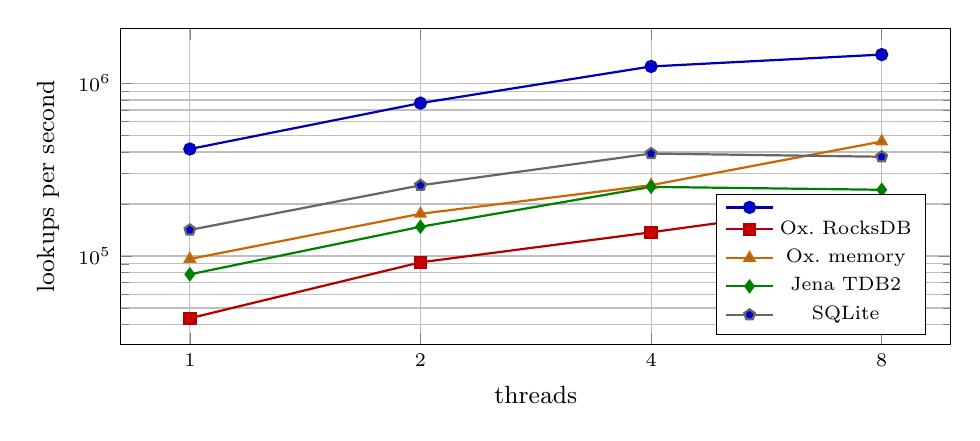
\begin{tikzpicture}
\begin{axis}[width=\columnwidth,height=5.6cm,xmode=log,ymode=log,log basis x=2,xtick={1,2,4,8},xticklabels={1,2,4,8},xlabel={threads},ylabel={lookups per second},grid=both,legend pos=south east,legend style={font=\scriptsize},tick label style={font=\scriptsize},label style={font=\small}]
\addplot+[mark=*,color=blue!70!black,thick] coordinates {(1,416050) (2,767222) (4,1250348) (8,1464779)};
\addlegendentry{\sys{}}
\addplot+[mark=square*,color=red!70!black,thick] coordinates {(1,43594) (2,91866) (4,137110) (8,208977)};
\addlegendentry{Ox.\ RocksDB}
\addplot+[mark=triangle*,color=orange!80!black,thick] coordinates {(1,96048) (2,175432) (4,256917) (8,459776)};
\addlegendentry{Ox.\ memory}
\addplot+[mark=diamond*,color=green!50!black,thick] coordinates {(1,78280) (2,147564) (4,251154) (8,241599)};
\addlegendentry{Jena TDB2}
\addplot+[mark=pentagon*,color=black!60,thick] coordinates {(1,141488) (2,256339) (4,391720) (8,375194)};
\addlegendentry{SQLite}
\end{axis}
\end{tikzpicture}

\caption{Lookups per second on LUBM(10) against threads (log-log).}
\label{fig-conc}
\end{figure}

\begin{table}[t]
\caption{Concurrency on LUBM(10): lookups per second with 1 and 8 reader threads, readers' lookups per second with one writer running, and inserts per second with 1 and 8 writer threads (one triple per transaction; \sys's inserts are not logged, and Jena's commit forces the journal to disk). The machine has 8 performance cores.}
\label{tab-conc}
\small
\resizebox{\columnwidth}{!}{%
\begin{tabular}{@{}lrrrrrr@{}}
\toprule
 & \multicolumn{2}{c}{lookups/s} & \multicolumn{2}{c}{readers + 1 writer} & \multicolumn{2}{c}{inserts/s} \\
\cmidrule(lr){2-3}\cmidrule(lr){4-5}\cmidrule(lr){6-7}
Engine & 1 & 8 & 1 & 8 & 1 & 8 \\
\midrule
\sys{} & 416k & 1.46M & 398k & 1.39M & 264k & 950k \\
Ox.\ RocksDB & 44k & 209k & 38k & 136k & 91k & 105k \\
Ox.\ memory & 96k & 460k & 69k & 288k & 679k & 186k \\
Jena TDB2 & 78k & 242k & 22k & 74k & 16 & 15 \\
SQLite & 141k & 375k & 111k & 322k & 15k & 14k \\
\bottomrule
\end{tabular}}
\end{table}


\stitle{Readers}.
\sys serves 416 thousand lookups per second with one thread and 1.46 million with
eight, 3.5 times more, and its one thread already beats every other engine at
eight except Oxigraph in memory (460 thousand); at eight threads it serves 7.0,
3.2, 6.1, and 3.9 times the lookups of Oxigraph on RocksDB, Oxigraph in memory,
Jena, and SQLite.
\stitle{Beside a writer}.
Its eight readers still serve 1.39 million lookups per second while the writer
inserts 111 thousand triples per second, 4.3 to 18.8 times the readers of the
other engines.
\stitle{Writers}.
\sys's insert rate grows 3.6 times, from 264 to 950 thousand per second; its
inserts bypass the write-ahead log here, while the others commit with their
default durability, and Oxigraph's in-memory store inserts faster with one thread
(679 thousand).
Heavy queries scale less: a 16,000-row query goes from 148 to 330 per second
with eight threads, bound by memory traffic.

\subsection{RQ4: Semantic Search}

\begin{table}[t]
\caption{Vector indexes on GO (recall@10, mean time per query, memory of the structure, build time).}
\label{tab-knn}
\small
\resizebox{\columnwidth}{!}{%
\begin{tabular}{@{}llrrrr@{}}
\toprule
Index & setting & recall & $\mu$s & MiB & build (s) \\
\midrule
flat float32 & exact & 1.000 & 2,238 & 55.8 & --- \\
flat 8-bit & exact over codes & 0.996 & 4,554 & 14.1 & --- \\
flat PQ $m{=}48$ & codes only & 0.778 & 819 & 1.7 & 10.4 \\
flat PQ $m{=}48$ & re-rank 100 & 0.998 & 905 & 1.7$^\dagger$ & 10.4 \\
IVF $\nu{=}512$ & $\rho{=}8$ & 0.892 & 149 & 56.5 & 17.5 \\
IVF $\nu{=}512$ & $\rho{=}16$ & 0.929 & 255 & 56.5 & 17.5 \\
IVF $\nu{=}512$ & $\rho{=}64$ & 0.976 & 928 & 56.5 & 17.5 \\
IVF $\nu{=}512$, 8-bit & $\rho{=}16$ & 0.926 & 263 & 14.8 & 17.5 \\
IVF $\nu{=}512$, PQ 96 & $\rho{=}16$ & 0.839 & 178 & 4.2 & 38.4 \\
HNSW $M{=}16$ & $\ef{=}10$ & 0.993 & 44 & 59.7 & 15.0 \\
HNSW $M{=}16$ & $\ef{=}40$ & 0.997 & 108 & 59.7 & 15.0 \\
HNSW $M{=}32$ & $\ef{=}160$ & 0.999 & 474 & 63.4 & 28.0 \\
\bottomrule
\end{tabular}}

\smallskip
{\footnotesize $^\dagger$ re-ranking reads the float vectors as well.}
\end{table}


\begin{figure}[t]
\centering
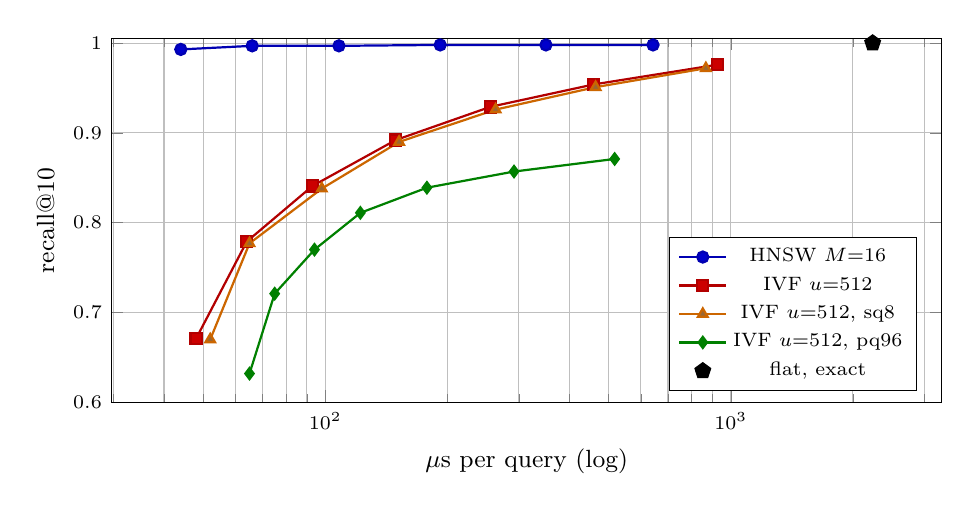
\begin{tikzpicture}
\begin{axis}[width=\columnwidth,height=6.2cm,xmode=log,xlabel={$\mu$s per query (log)},ylabel={recall@10},ymin=0.6,ymax=1.005,grid=both,legend pos=south east,legend style={font=\scriptsize},tick label style={font=\scriptsize},label style={font=\small}]
\addplot+[mark=*,color=blue!70!black,thick] coordinates {(44,0.993) (66,0.997) (108,0.997) (192,0.998) (350,0.998) (643,0.998)};
\addlegendentry{HNSW $M{=}16$}
\addplot+[mark=square*,color=red!70!black,thick] coordinates {(48,0.671) (64,0.779) (93,0.841) (149,0.892) (255,0.929) (459,0.954) (928,0.976)};
\addlegendentry{IVF $
u{=}512$}
\addplot+[mark=triangle*,color=orange!80!black,thick] coordinates {(52,0.67) (65,0.777) (98,0.838) (152,0.89) (263,0.926) (464,0.951) (868,0.972)};
\addlegendentry{IVF $
u{=}512$, sq8}
\addplot+[mark=diamond*,color=green!50!black,thick] coordinates {(65,0.632) (75,0.721) (94,0.77) (122,0.811) (178,0.839) (292,0.857) (517,0.871)};
\addlegendentry{IVF $
u{=}512$, pq96}
\addplot[only marks,mark=pentagon*,mark size=3pt,color=black] coordinates {(2238,1)};
\addlegendentry{flat, exact}
\end{axis}
\end{tikzpicture}

\caption{Recall@10 against time per query on GO (38,092 vectors, 384 dimensions).}
\label{fig-knn}
\end{figure}


On 38,092 Gene Ontology terms and 1,000 queries (Table~\ref{tab-knn}, Figure~\ref{fig-knn}), HNSW ($M{=}16$) reaches recall
0.993 at 44\,$\mu$s, 51 times faster than the 2.2\,ms exact scan, for 3.9\,MiB of
links; IVF over the B+ tree ($\nu{=}512$) needs 255\,$\mu$s for 0.929 and
928\,$\mu$s for 0.976, about 2.7$\times$ the cost per scored row of a contiguous
scan, the price of lists that page, cache, and update with the triples.
Our first exact baseline used a scalar loop the compiler would not vectorize and
took 8.3\,ms, which would have doubled every speed-up; we report against the
vectorized 2.2\,ms.

\begin{table}[t]
\caption{Ten nearest terms under a class $c$: recall@10 / $\mu$s per query, for a query inside or outside $c$ and classes with at most 10 or more than 5,000 members (Gene Ontology). Bold marks the fastest exact or near-exact strategy.}
\label{tab-hybrid}
\small
\resizebox{\columnwidth}{!}{%
\begin{tabular}{@{}lcccc@{}}
\toprule
 & \multicolumn{2}{c}{query inside $c$} & \multicolumn{2}{c}{query outside $c$} \\
\cmidrule(lr){2-3}\cmidrule(lr){4-5}
Strategy & $\le$10 & $>$5,000 & $\le$10 & $>$5,000 \\
\midrule
pre-filter, exact & \textbf{1.00 / 3} & 1.00 / 1,404 & \textbf{1.00 / 3} & 1.00 / 1,394 \\
post-filter, IVF & 0.86 / 903 & 0.99 / 211 & 0.07 / 966 & 0.64 / 591 \\
masked HNSW & 1.00 / 16,653 & \textbf{1.00 / 105} & 1.00 / 16,802 & \textbf{1.00 / 900} \\
auto (threshold 4,096) & \textbf{1.00 / 3} & \textbf{1.00 / 95} & \textbf{1.00 / 3} & \textbf{1.00 / 860} \\
\bottomrule
\end{tabular}}
\end{table}

\stitle{Exact pre-filtering for small classes, masked search for large}.
Up to about 1,000 members, resolving the members through the intervals and scoring
them exactly takes 3 to 62\,$\mu$s and is the exact answer, $10^2$ to $10^4$
times faster than any index strategy.
Post-filtering fails for outside queries (IVF recall 0.07 on the smallest classes,
0.64 on the largest); above 5,000 members masked HNSW takes 105 to 900\,$\mu$s,
exact, against 1.4\,ms for resolving and scoring.
With a threshold of 4,096 members, auto matches the fastest strategy in every cell
but one and is never slower than 0.9\,ms; the cell it loses (269\,$\mu$s against
70\,$\mu$s) avoids a factor of 79 in its neighbor.
